% !TEX root = ../../../main.tex
% 来源：中学数学实验教材·第二册（几何）
% 章节：集合与简易逻辑 / 简易逻辑
% 原始文件：2.tex，行 1763-1771
% 类型：tikz
% ---
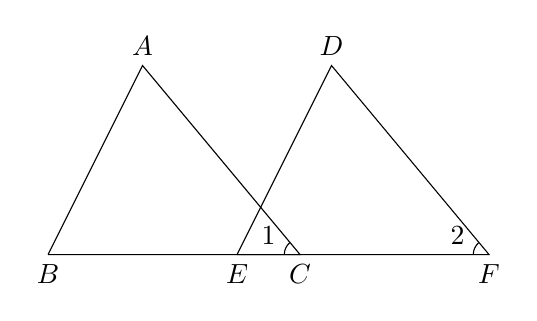
\begin{tikzpicture}[>=latex, scale=.8]
\draw (0,0)node[below]{$B$}--(4,0)node[below]{$C$}--(1.5,3)node[above]{$A$}--(0,0);
\draw (3,0)node[below]{$E$}--(7,0)node[below]{$F$}--(4.5,3)node[above]{$D$}--(3,0);
\foreach \x/\xtext in {4/1,7/2}
{
	\draw (\x-.25,0) arc (180:130:.25);
	\draw(\x-.5,0)node[above]{$\xtext$};
}
    \end{tikzpicture}
